\documentclass[]{article}

% Review comments stuff
% -----------------------------------------
\usepackage[english]{babel}
\usepackage[dvipsnames,svgnames,x11names]{xcolor}
\usepackage[markup=underlined]{changes}
% Use "final" option to remove all tracking markups
% \usepackage[final]{changes}

\definechangesauthor[color=BrickRed]{RB}

% Alternative definition to have the remarks
% in the margins instead of footnotes
\usepackage{todonotes}
\setlength{\marginparwidth}{3cm}
\makeatletter
\setremarkmarkup{\todo[color=Changes@Color#1!20,size=\scriptsize]{#1: #2}}
\makeatother

%% Definition of a plain remark/note
\newcommand{\note}[2][]{\added[#1,remark={#2}]{}}

% -----------------------------------------

% Increase text width
\usepackage[left=48pt,right=46pt]{geometry}

% Graphics Stuff
\usepackage{graphicx}
\usepackage{float}
\graphicspath{ {images/} }

% Bibliography stuff
\usepackage[round]{natbib}
% Adds bibliography to toc
\usepackage[nottoc,numbib]{tocbibind} 

% Makes toc, urls, figure links
\usepackage{hyperref}

% Format hyperlinks nicer than default way
\usepackage{xcolor}
\hypersetup{colorlinks,linkcolor={blue!80!black},citecolor={blue!80!black},urlcolor={blue!80!black}}

% Define custom lists
\usepackage{enumitem}
\newlist{AO}{enumerate}{1}
\setlist[AO,1]{label = \textbf{AO\arabic*}}

\newlist{POC}{enumerate}{1}
\setlist[POC,1]{label = \textbf{POC\arabic*}}


% Title Page
\title{Backup Management and Orchestration System\\
	Final Year Project}
\author{Rob Shelly\\
	Applied Computing\\
	20068406}

\begin{document}
%\maketitle
% Use custom title page to adhere to project manual
\noindent \LARGE{\textbf{Backup Restoration Test System}}
\bigbreak
\noindent \large{Status Report (semester 1)}
\bigbreak
\noindent \Large{Rob Shelly}
\bigbreak
\noindent \Large{20068406}
\bigbreak
\noindent \Large{Supervisor: Dr. Rosanne Birney}
\bigbreak
\bigbreak
\noindent \Large{BSc (Hons) in Applied Computing}
\thispagestyle{empty}

\newpage
\pagenumbering{roman}
\tableofcontents

\newpage
\pagenumbering{arabic}
\section{Introduction}

\subsection{Problem Statement}
In January 2017 GitLab suffered a data loss incident which was widely reported in the media. It began with spammers targeting GitLab.com and culminated in an engineer erroneously deleting 300GB of PostgreSQL data in a production environment. The lost data included merger requests, users and comments \citep{gitlab1}. The bigger story was to come later however when it was realised that GitLab's backup process had failed silently. The backups did not exist, thus resulting in a total loss of the data. As it transpired, conflicting major versions of \textit{pg\_dump} (a utility for backing up PostgreSQL databases) in use for the backup procedure and the PostgreSQL database resulted in an error, and the procedure failing \citep{gitlab2}.

The incident was widely reported in the tech industry with the story being picked up by a number of outlets including TechCrunch \citeyearpar{lomas} and The Register \citeyearpar{sharwood}. For many, the focal point of the story was the failed backups. The incident highlighted the need for regular verification of backups. A simple way of performing this verification is to regularly restore data. The method of verification is to perform a restore of the data, which can be a mundane and time consuming task. The aim of this project is to create a solution to the issue. A system which can notify administrators when backups have failed may have prevented the data loss in the GitLab ordeal.

\subsection{Aims \& Objectives}
The overall objective is to create a system to test that uncorrupted backups exist and contain valid, readable data. A system will be created that allows sysadmins to test backups and to schedule the regular testing of backups. This will be achieved by performing restoration on the backups. The main objectives of the system are as follows:

\begin{AO}
	\item \label{ao1} Eliminate the mundane and time consuming task of backup testing by automating regular backup restorations and recording results;
	\item \label{ao2} Catch silent failures of the backup procedure by notifying sysadmins of failed backups;
	\item \label{ao3} Reduce the cost of backup restoration testing by automating the process of creating the necessary infrastructure (such as virtual machines on AWS), performing the restoration and destroying the infrastructure once results are obtained, thus minimising the uptime of infrastructure;
	\item \label{ao4} Perform the restoration check in a secure manner by managing encryption keys and the movement and decryption of data only when necessary in safe environment.
\end{AO}

The system will focus on backups of databases. For scope, design will focus on testing MongoDB data and MySQL data, thereby providing a sample of both relational and non-relational database management systems (DBMS). However, the system should be designed such that it can be easily modified to test data from others forms of database management systems. As part of the system, the following should be implemented:

\begin{itemize}
	\item \textbf{Web app:} This will act as a front end for the sysadmins to run and schedule tests and view results.
	\item \textbf{Automation Server:} This will be the backend of the system. It will take care of retrieving the backup data before performing some sorts of tests.
	\item \textbf{Container Platform:} This will be utilised by the backend to test the server. For example, when testing the data from a MongoDB database, the backend will spin up a container with MongoDB installed in order to verify the data. 
\end{itemize}

\section{Semester One Summary}
Semester one consisted of the research phase of this project. As part of the research phase, the technical feasibility of the project was assessed by first defining the following three \textit{Proof of Concepts}:


\begin{POC}
	\item \label{poc1} \textbf{Validation:} How will a restoration be validated? What criteria are needed for a backup to be deemed successful?
	\item \label{poc2} \textbf{User Rules:} How will a user use the system? Can the the implementation of a backup restoration be abstracted from the user by means of a user friendly frontend?
	\item \label{poc3} \textbf{Security:} How will the system deal with encrypted backups? Can the Jenkins server safely handle credentials and decrypt backups in order to perform the test restoration?
\end{POC}

\subsection{\ref{poc1} Validation}
  This POC was test by creating a Jenkins job which restores a backup file to the DBMS and perform a full read of the database.

	\subsubsection{Work Completed}
	In order to prove that validation can be achieved via Jenkins the following infrastructure was deployed to AWS:
	\begin{itemize}
		\item \textbf{Backup Server:} An EC2 instance on which a backup file was saved.
		\item \textbf{Restoration Server:} An EC2 instance with the MongoDB DBMS installed and running.
		\item \textbf{Jenkins Server.}
	\end{itemize}
	A Jenkins job was then configured to execute the following tasks:
	\begin{enumerate}
		\item Copy backup file from \textit{backup} server to \textit{restoration} server (sample MongoDB data used \citep{mongo});
		\item Import the backup file into MongoDB on \textit{restoration} server;
		\item Run a \textit{findAll} command on the MongoDB database to retrieve all entries;
		\item Print the entries to Jenkins console;
	\end{enumerate}

	\subsubsection{Results}
  The POC showed backups can be successfully transported to and imported into a remote server. Once imported, a successful \textit{findAll} command proves that the data is still readable. The POC also demonstrated that a the SSH credentials for the various servers could be stored in Jenkins and used securely into order connect to them.
  
\subsection{\ref{poc2} User Rules}
	This POC was tested by creating a basic frontend with React which uses Jenkins API to trigger an arbitrary Jenkins Job.
	
	\subsubsection{Work Completed}
  The following tools were utilised to create a web interface for Jenkins.
  \begin{itemize}
    \item A basic web app was created with ReactJS, consisting of a simple form to input parameters;
    \item A parameterised Jenkins job was;
    \item The NodeJS wrapper for the Jenkins API, which allows Jenkins API calls to be made with NodeJS.
  \end{itemize}
  When the web form was completed and submitted, the web app trigger the parameterised job (including the parameters input to the form) via the api.

  \subsubsection{Results}
  The POC demonstrated that implementation of Jenkins jobs can be abstracted from the user therefore allowing the system to present the user with a simple form to complete in order to commence an automated restoration.

\subsection{\ref{poc3} Security}
  This POC was tested using the same AWS infrastructure as \hyperref[poc1]{POC1}. In this instance, the backup file had been encrypted with a GPG.

  \subsubsection{Work Completed}
	In this instance the Jenkins job copied the encrypted backup to the \textit{restoration} server. The backup was then decrypted using GPG and a private key on the \textit{restoration} server and the contents printed to verify decryption. 
	
  \subsubsection{Results}
  This POC demonstrated that the system, in it's current architecture, can successfully copy an encrypted backup file to the \textit{restoration} server where it is decrypted. It also demonstrated that the GPG private keys can be securely stored and used by Jenkins.

  \subsection{Prototype}
  As a final task, the three POCs were integrated to create a prototype. The prototype consisted of a single form on a web app which allowed the user to inupt the IP address or DNS and filename of a encrypted backup file. When the form was submitted, it triggered a Jenkins job which moved the file to a restoration server where it decrypted the file. It then import the file into a DBMS and preformed a full read of the database, thereby proving that the backup file was valid.


\section{Technologies}

\subsection{Docker}
Docker is a container platform for building and managing applications. This project is interested not in Dockers platform but rather in the Docker images that run on the platform. A container image is a modular piece of software. It encapsulates all the code and tools needed to run the software packaged in the image. The image can then be run in a container on any environment using a container platform or service. Thus, it runs independent of the hardware or operating system. The container also isolates the software from other images and software running within the environment \citep{docker}.

The ability to build applications as OS agnostic images makes is appealing for this project. It allows the frontend application to be built as an image and run on any system running Docker, for example an AWS EC2 instance. 


\subsection{Amazon Web Services}
The project will make extensive use of Amazon Web Services (AWS) with most or possibly all of the systems infrastructure deployed on AWS, particularly using EC2 and ECS.

EC2 is Amazon's compute service. It allows easy deployment and management of virtual compute resources within the cloud. The flexibility of operating systems, virtual machines (or instances as they are known in AWS) and size of volume of storage make it ideal for this project \citep{ec2}. It will allow the system to create instances with only the necessary resources required (i.e. memory and storage) to test the restoration of a given backup. This keeps the cost of testing to a minimum in keeping with Aim \ref{ao3}.

ECS is Amazon's container management service. It allows Docker images to be easily deployed to and run on  EC2 instances, taking care of Docker installation and management, for example managing port mappings between containers and the host. There is no added cost for using ECS. i.e. the customer only pays for the EC2 instances \citep{ecs}. 

\label{aws-cli} AWS also features a command line interface for building, modifying and destroying infrastructure across all of it's services, providing a programmatic method of creating the resources. The ability to do so allows for the automation of the infrastructure creation and destruction. This makes AWS an ideal platform for this project as automation is an objective of the project set out in Aim \ref{ao1}. 


\subsection{Jenkins}
Jenkins is an automated build server used to implement continuous integration (CI) and continuous delivery (CD). Configuration and management of the server can be achieved using both a web interface and an API. Jenkins is also extensible through a library of plugins \citep{jenkins}.
 
Jenkins was chosen as a backend service for this project as it, along with it's library of plugins, presents many useful features which will be beneficial to the implementation of the system:
\begin{itemize}
	\item A built in email notification system which can be used to notify users of silently failed backups. This provided the functionality to implement a satisfactory solution to Aim \ref{ao2};
	\item \label{creds-plugin}A Credentials plugin which provides a means of storing various credentials in various forms (e.g. username/password pairs, SSH keys) along with a standard API for Jenkins and other plugins to access and use these credentials \citep{connolly}. This provides a secure manner for using SSH keys for backup servers. This is a key objective of the project outlined in Aim \ref{ao4}.
	\item The ability to schedule jobs to run at regular intervals will provide the functionality described in Aim \ref{ao1}. This eliminates the need for the development of a scheduling system. 
	\item The REST API can be used by a user-friendly web based frontend, allowing users unfamiliar with Jenkins or AWS to perform test restorations. 
\end{itemize}


\subsection{Node}
The frontend of the system will be designed using Node (also known as Node.js). Node is a JavaScript runtime environment for building network applications. It is light-weight and efficient framework through its event driven, no blocking I/O implementation. 

The default package manager of Node is \textit{npm} (for Node Package manager). It is the worlds largest software registry \citep{npm}. The vast registry of free and open source packages available make Node an attractive choice for this project. Of particular interest are the multiple Node clients for Jenkins. These are Node wrappers for the Jenkins REST API enabling easy integration of the frontend with the Jenkins backend.

Although any of a number of frameworks could have been used, for example Django, Node was chosen for this project due it's light-weight design and extensibility through \textit{npm}, including the aforementioned Jenkins API wrappers.
 
\subsection{React}
The UI element of the frontend will be built using React, a JavaScript library available through \textit{npm} for building user interfaces. React is developed to work independently of other technologies, meaning it can be integrated easily with Node and other \textit{npm} packages without the need for refactoring. React builds UIs as a set of components, each managing their own state and implementing their own render function. This allows fast and efficient rendering of data changes as only components that are updated will be re-rendered.


\section{Design}
	\subsection{System Architecture Overview}
		The system will comprise of three main components:
		\begin{itemize}
			\item Management Server
			\item User Interface
			\item Disposable instances/containers
		\end{itemize}
		The system will also use existing ECS instances i.e  where backups are stored. Depending on the user of the system there may be multiple backup servers in different location (such as AWS regions) or for different data types (relational and non-relational databases).
		
		\begin{figure}[H]
			\setlength{\belowcaptionskip}{15pt plus 3pt minus 2pt}
			\caption{Diagram of System Architecture}
			\centering
			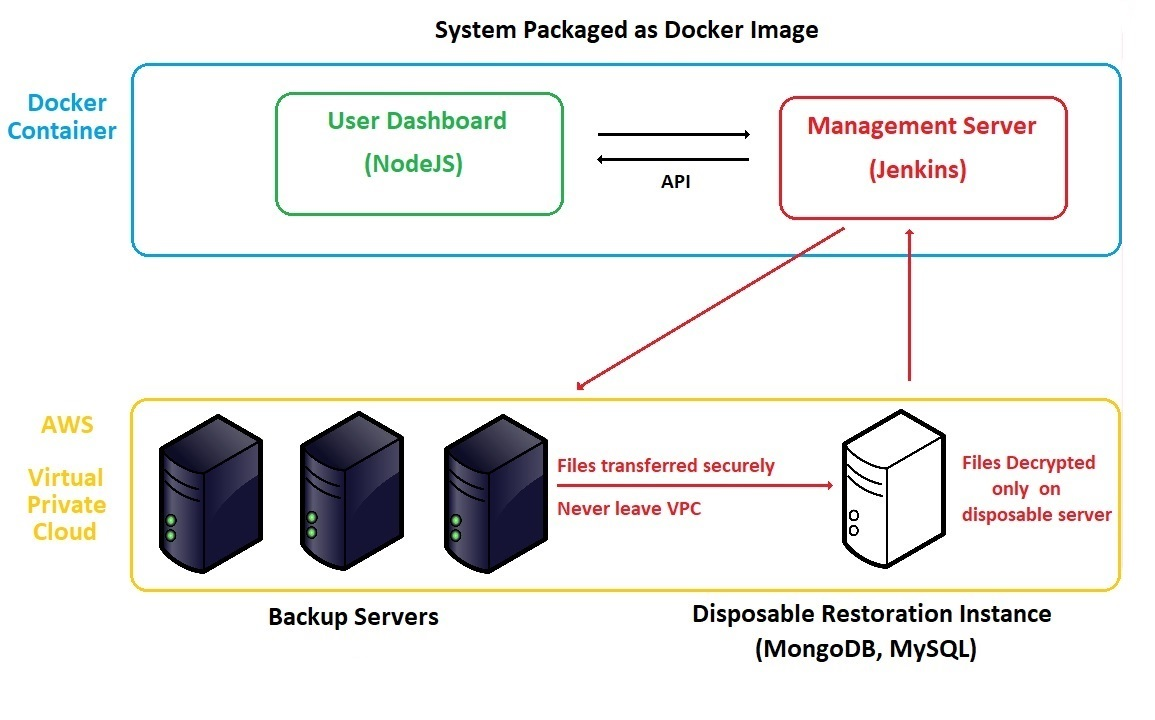
\includegraphics[scale=0.5,keepaspectratio]{system-architecture}
			\label{fig:diagram}
		\end{figure}
		
		\noindent \textbf{Management Server:} This will be a small low cost AWS instance on which the Jenkins automation server will be installed. The majority of the system's functionality will be carried out and/or orchestrated by this server. Jenkins jobs will copy the backups from their location to a disposable instance and implement the necessary steps to validate them such as importing and and reading.
		
		\noindent \textbf{User Interface:} This will provide a simple user interface (UI) for the system, implemented as a simple web app, hosted on AWS. It will allow users with little knowledge of Jenkins and AWS to perform backup restoration checks by adding a layer of abstraction. Users will be able to run restorations by providing the parameters such as the backup file and its location. The UI will utilise the Jenkins API to execute the restoration with the parameters provided.
		
		\noindent\textbf{Disposable Instances:} Disposable infrastructure will be used to perform the restoration. This will consist of EC2 instances running the necessary DBMS to perform the restoration. They can also be destroyed afterwards, destroying the data and therefore maintaining confidentiality.

	\subsection{Formal Modelling}
	\subsubsection{Sequence Diagrams}
		The main function of the systems have been demonstrated below in sequence diagrams. \autoref{fig:seq-run-restore} shows the process of running a single backup restore. This involves a user manually triggering a restoration using the web interface. This triggers a Jenkins job which automates the remaining steps:
		\begin{enumerate}
			\item Backup copied to \textit{restoration} server;
			\item Backup decrypted;
			\item Backup import into DBMS;
			\item Data read from DB;
		\end{enumerate}
		Upon completion the \textit{restoration} server is terminated.

		\autoref{fig:seq-schedule-restore} shows the process of a scheduling regular backup restoration tests. Again, this is triggered by a user from the web interface. The web interface will pass the JSON or XML configuration for a job to the Jenkins server. The server verify the backup server exists before creating the job.
		
		\autoref{fig:seq-delete-restore} Show the process of deleting an existing scheduled job. The user triggers this process from the web interface. This sends a delete commands to the Jenkins server via the API to remove the schedule job. The status of the command, indicating a successful or failed restore, is returned to the user.
		
		\begin{figure}[H]
			\setlength{\belowcaptionskip}{15pt plus 3pt minus 2pt}
			\caption{Run Restore}
			\centering
			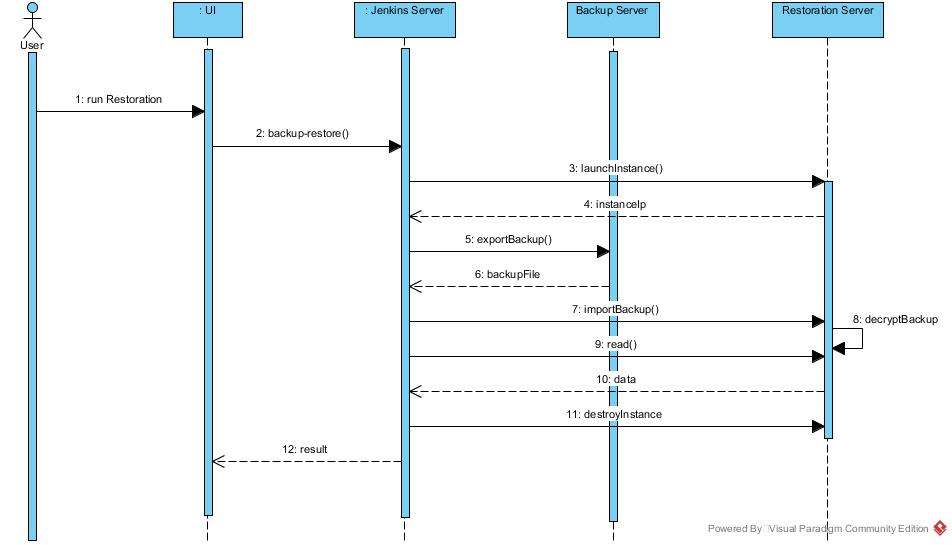
\includegraphics[width=\textwidth,keepaspectratio]{sequence-diagram-run-restore}
			\label{fig:seq-run-restore}
		\end{figure}
		
		\begin{figure}[H]
			\setlength{\belowcaptionskip}{15pt plus 3pt minus 2pt}
			\caption{Schedule Regular Restore}
			\centering
			%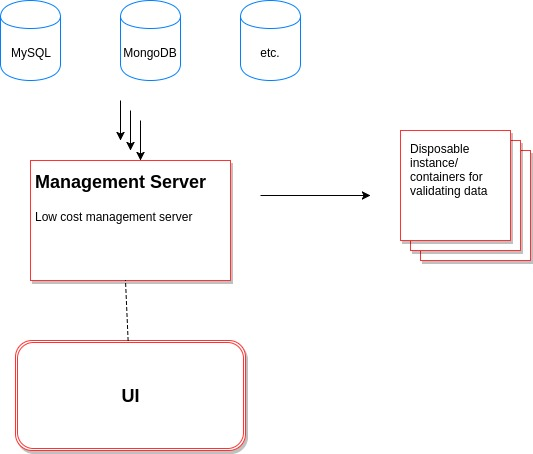
\includegraphics[width=\textwidth,height=\textheight,keepaspectratio]{diagram}
			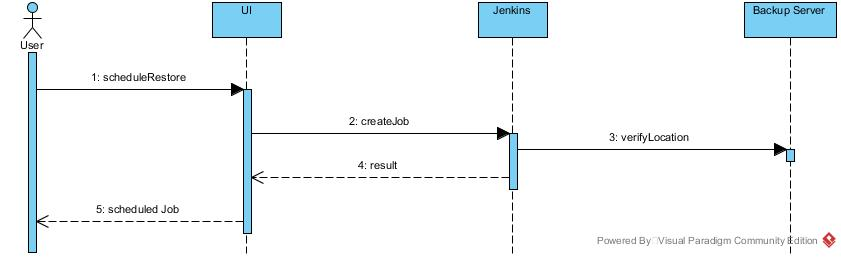
\includegraphics[width=\textwidth,keepaspectratio]{sequence-diagram-schedule-restore}
			\label{fig:seq-schedule-restore}
		\end{figure}
		
		\begin{figure}[H]
			\setlength{\belowcaptionskip}{15pt plus 3pt minus 2pt}
			\caption{Delete Scheduled Restore}
			\centering
			%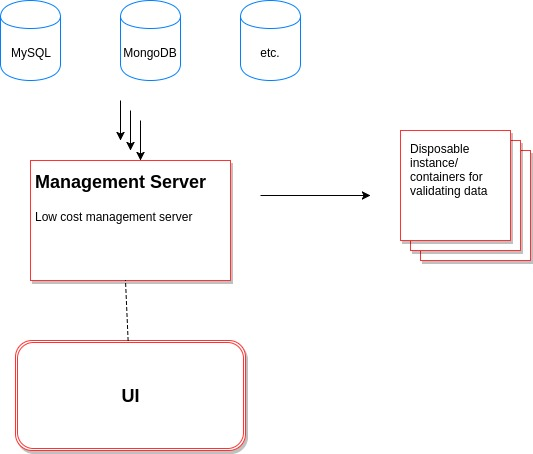
\includegraphics[width=\textwidth,height=\textheight,keepaspectratio]{diagram}
			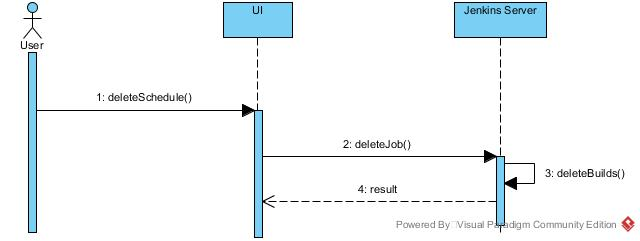
\includegraphics[width=\textwidth,keepaspectratio]{sequence-diagram-delete-schedule}
			\label{fig:seq-delete-restore}
		\end{figure}
	
	\subsubsection{User Stories} \label{user-stories}
   
		User stories are provided in \autoref{table:user-stories}. Two types of system users and their privileges are described below;
		
		\textbf{Managers} control security aspects of the system:
		\begin{itemize}
			\item Add and remove regular users;
			\item Manage SSH keys and decryption keys.
		\end{itemize}
		\textbf{Regular Users} will perform the day-to-day tasks of the system:
		\begin{itemize}
			\item Perform restorations;
			\item Schedule restorations;
			\item View restoration results;
		\end{itemize}
		
		\begin{table}[H]
			\small
			\centering
			\setlength{\belowcaptionskip}{15pt plus 3pt minus 2pt}
			\caption{User Stories}
                         
			\begin{tabular}{|l|l|p{0.39\linewidth}|p{0.39\linewidth}|} \hline
				\textbf{\#} & \textbf{As a} & \textbf{I want to be able to} & \textbf{so that} \\ \hline
				US1 & manager & implement a user system & I control who can run backup restores \\ \hline
				US1.1 & manager & add my team members to the system & they can run backup restores \\ \hline
				US1.2 & manager & remove users from the system & former team members no longer have access \\ \hline
				US2 & manager & add and control sensitive information within the system & I can implement a security policy \\ \hline
				US2.2 & manager & securely store credentials within the system & they don't need to be entered every time a restore is executed \\ \hline
				US2.3 & manager & add SSH keys for backup server & the system has secure access backup server \\ \hline
				US2.4 & manager & add decryption keys for backups & encrypted backups can be decrypted for testing \\ \hline
				US2.5 & manager & delete SSH keys & expired/outdated credentials are no longer stored \\ \hline
				US2.6 & manager & delete decryption keys & expired/outdated credentials are no longer stored \\ \hline
				US3 & manager & execute all same tasks as a regular user & I don't need a second set of credentials to run restores myself \\ \hline
				US4 & user & login & I can run restores \\ \hline
				US5 & user & logout & I avoid potential unauthorised access \\ \hline
				US6 & user & run a test restoration of a backup & I can verify that the backup exists, is a valid file, and is readable \\ \hline
				US6.1 & user & run a test by filling out a simple form with basic parameters (location, filename) of the backup to test & I can easily run a restore of a specific backup without needing to worry about the implementation \\ \hline
				US6.2 & user & view the current status of a running restoration & I can review the progress of long running restores \\ \hline
				US6.3 & user & check if a backup failed or succeeded & I can immediately investigate any failed backups \\ \hline
				US7 & user & create a schedule of automated restores for a given backup & I don't have to manually execute them myself on a regular basis \\ \hline
				US7.1 & user & choose the frequency of automated restores within a schedule, from daily through weekly to monthly & I control how often different backups are tested \\ \hline
				US7.2 & user & check if an automated restoration has started & I can verify my schedule is working correctly \\ \hline
				US7.3 & user & check the results of an automated restore & I can immediately investigate any failed backups \\ \hline
				US7.4 & user & view the all past results of an automated restore schedule & view the consistency of my backups success \\ \hline
				US7.5 & user & modify a scheduled restore & I can change the frequency of a scheduled restore \\ \hline
				US7.6 & user & the parameters of a schedule & any changes to the backups, such as location, will be reflect in the restoration schedule \\ \hline
				US7.7 & user & delete regularly scheduled restores & old backups/deleted backups are no longer tested \\ \hline 
				US8 & user & view feedback of a failed restore & I might gain an insight into the fault in the backup \\ \hline
				US9 & user & notified when a restoration fails & silent, unnoticed fails are avoided \\ \hline
			\end{tabular}
			\label{table:user-stories}
		\end{table}
		

        
	\subsection{Front End Design}
	\subsubsection{Wireframes}
	
		Wireframes for the frontend are shown below. 
        
        \autoref{fig:homepage} shows the homepage. It includes the following components:
		\begin{itemize}
			\item Form for running a restore;
			\item Form for creating a restore schedule;
			\item List of schedules (including links).
		\end{itemize}
		\autoref{fig:scheduled} shows the details and past results of a scheduled restore.
		
		
		\begin{figure}[H]
			\setlength{\belowcaptionskip}{15pt plus 3pt minus 2pt}
			\caption{Homepage}
			\centering
			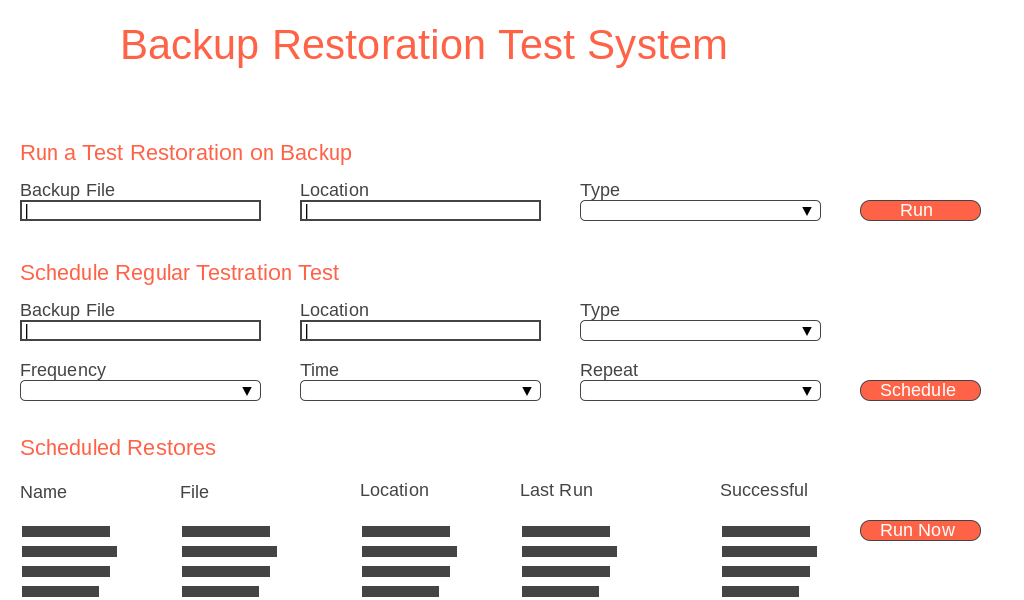
\includegraphics[width=\textwidth,keepaspectratio]{wireframe-homepage}
			\label{fig:homepage}
		\end{figure}
		
		\begin{figure}[H]
			\setlength{\belowcaptionskip}{15pt plus 3pt minus 2pt}
			\caption{Scheduled Restore}
			\centering
			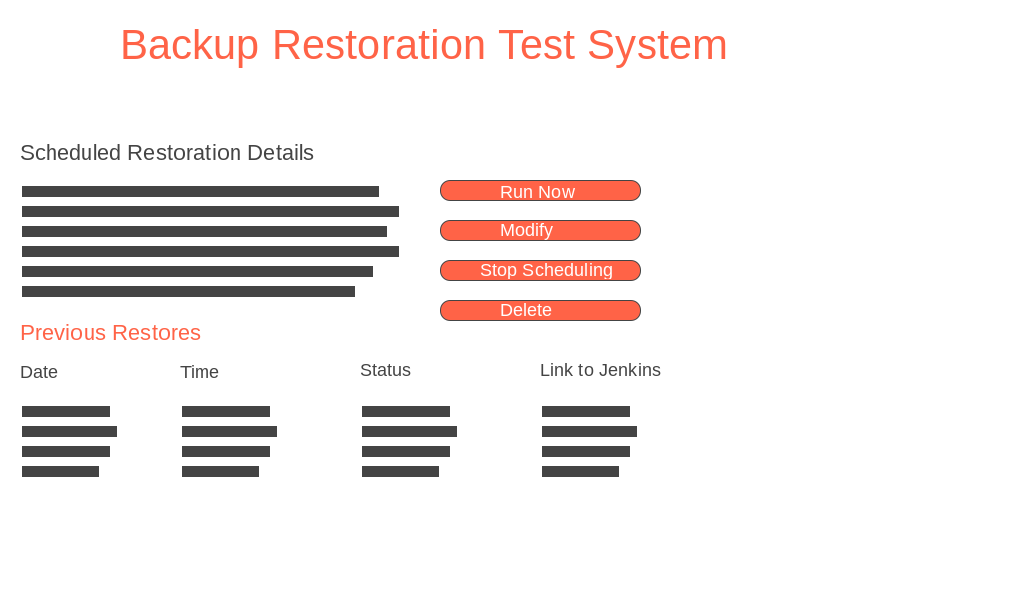
\includegraphics[width=\textwidth,keepaspectratio]{wireframe-scheduled-restore}
			\label{fig:scheduled}
		\end{figure}

	\subsection{Enterprise Level Consideration}
  As this project is being designed for the product owners to potentially deploy it to test production database backups there are a number of key aspects which should be considered. This is to ensure the product does not just achieved it's main goals but does so in a secure and useable manner for the product owners.
  
  \subsubsection{Security}
  Security is a key aspects of this project. In fact , due to the importance of security it has been defined as one of the key aims of the project (\hyperref[ao4]{AO4}). The security of this system shall by determined by two main areas.
  
  \subsubsubsection{Storage of Private Keys}
  This pertains the storage of the SSH private keys for accessing backup servers and the GPG private keys used to decrypt the backups. Safe storage of such keys is paramount to the project as exposing these keys would comprise production data. Accordingly, during the research phase of the project, \hyperref[poc3]{POC3} was concerned with investigation this area.
  In this POC, Jenkins Credentials Plugin was used to stored the credentials. A prototype was then used to to demonstrated that the private keys could be used to implement a backup restoration while maintain the confidentiality of the keys.
  
  \subsubsubsection{User Authentication}
  Users of the system will not be able to retrieve any sensitive data through it's use rather they will be ability to schedule and run backup restorations. Restorations do not affect the existing backup files or servers, rather completing the test restoration on a disposable server in AWS. Also restorations are idempotent, so running more than one test on a given backup wont affect the results.
  
  Therefore, malicious users of the system could not affect data confidentiality. However, they could incur increased AWS costs by running and scheduling extra restorations. For that reason access to the UI should be restricted.  Accordingly, a the implementation of a user authentication system has been added to the product backlog. However, it was decided that for the purposed of creating an Minimum Viable Product (MVP), user authentication should be prioritised rather low on the backlog as an final product would likely run in a private network or Virtual Private Cloud. However, user authentication will still be implemented for version two.
  
  \subsubsection{Deployment}
  During discussion with the product owners it was decided that the deployment on installation of the final product would be a simple task, requiring little or no configuration of the user. For this reason it was decided that the final product should be delivered as a Docker image.
  
  However, the final system consist of two servers; the management server (Jenkins) and a web server (UI). This means two services are required to run within the Docker image. However, this is not the recommended practice for Docker images \citep{docker2}. A container should be run as a single process which if terminated will terminate the container. For this reason the final product should be package as two images. These images can still be easily run with any configuration required. They will run in separate containers but are preconfigured to be able to communicate.
  
  This method of deploying systems as a network of containers is in fact a common practice in the industry, leading to the development of container management platforms such as Kubernetes \citep{kubernetes}. Accordingly, OpenShift, Red Hat's own container management platform has been considered as the suitable deployment location for the final product.
  
  \subsubsection{Performance}
  The use of containers to run the final products play a key rol in the performance of the system. Containers are similar to virtual machines allowing them to run ona variety of platforms. However, as containers virtualise software instead of hardware, they are much smaller and faster to run \citep{docker}.
  
  Packaging the final product as Docker images is therefore the suitable solution for implementing a high performance system. The images will contain, and therefore run, only the necessary software to run both the Jenkins server and the node app. Indeed, both the Jenkins server and app server can be easily run on a single device.
  
\section{Methodology}
	\subsection{Agile}
	The design methodology chosen for this project is Agile. Agile takes an iterative approach to designing and delivering products. It's a goal driven methodology that aims to build and deliver software incrementally from the beginning of the project, in contrast with traditional approaches such as Waterfall which deliver in one final stage. A notable aspect of Agile is user stories. The project is broken into small sections of functionality which can be independently developed and delivered upon completion \citep{rasmusson}. A number of user stories have been described \hyperref[user-stories]{above}, detailing the main requirements of this project. 
	
	\subsubsection{Scrum}
	
	A particular Agile framework which will be used for this project is Scrum. Scrum defines terms used to organise development:
	\begin{itemize}
		\item \textbf{Product Backlog:} This is a prioritised list of jobs which need to be completed. In its entirety, it represents the full development of the project, i.e. all the work required to deliver the final product.
		\item \textbf{Sprints:} Development is divided into a number of equal length periods (often two or three weeks) of work known as sprints. Each sprint has it's own small goal to achieve, with some items from the head of the product backlog being developed. This project will be organized into six sprints of two weeks each.
		\item \textbf{Daily Scrum:} The daily scrum, also known as daily \textit{standup}, is a daily meeting at which team members meet to discuss progress and address issues encountered.
		\item \textbf{Sprint Reviews:} At the end of each sprint a review of the work completed is carried out. The next sprint will then begin, developing the next group of items from the backlog being\citep{scrum}.
	\end{itemize}
	Also defined are a number of roles:
	\begin{itemize}
		\item \textbf{Product Owner:} The product owner is responsible for the backlog. They are responsible for ensuring the development succeeds in its goals by implementing the work laid out in the backlog. It is the duty of the product owner to prioritise the backlog. 
		\item \textbf{Scrum Master:} The scrum master is responsible for maintaining focus on the current batch of backlog items during each sprint \cite{agile}.
	\end{itemize}
	
	Scrum is an ideal model for developing this project. The Product Owner will be Reat
  d Hat and the role of scrum master will be played by the project supervisor. Development will broken into six sprints of two weeks. However, as this is not a team project, daily stand-up meetings will not be held. Rather, meetings with the scrum master on weekly basis and meetings with the product owner on a similar schedule as needed. The user stories which have been used to describe the requirements of the project will be organised into the product backlog.
	
	\subsection{Jira}
	In conjunction with the Scrum framework the Jira development tool will be used. Jira is a project management tool which allows the creation and tracking of tasks or issues. The product backlog, comprising of the project user stories, can be created within the management tool with tasks created for each of the stories on the backlog. Each task can then be prioritised as the in the manner chosen by the product owner \citep{jira}.
	
	A number of Jira's feature make it an ideal tool to aid in the organisation of this project:
	\begin{itemize}
		\item \textbf{Issue Tracking:} Progress on issues within the product backlog can be tracked though useful status tags such as In Progress, On Hold and Done. This provides a mechanism for recording progress on each of the user stories which implemented for this project. 
		\item \textbf{Scrum Boards: } Sprints can be represented using Scrum boards. Scrum boards provide a way of organising the issues in a visual manner, grouping them into logical categories (To Do, In Progress, Done) focus on the progress of the current sprint \cite{scruminc}.
	\end{itemize}

	\subsection{Continous Integration/Deployment}
	Continuous Integration/Continuous Deployment (or continuous Delivery) is a development concept that focuses on the frequent and automated testing building and releasing of code. It aims to remove the large workload required when it is time to release a version or update of a product by performing the same process in a automated manner on every code commit \citep{pittet}.
	
	Continuous integration refers to preparing the code for release as often as code commits are performed. For example, running tests and building Docker images on each commit meaning code is prepared for release at each stage of development, instead of when it come to release time \citep{ramos}.
	Continuous Deployment is a step beyond Continuous Integration. After the code is built it is deployed to a server. However, this may be a development server. Pushing the built code to production requires a manual trigger. Continuous Delivery automates this final manual trigger, meaning the entire process of moving code through testing, building and deployment to production is entirely automated \citep{ellingwood}.
	
	For this project, CI/CD (continuous development in this case) will be implemented using a Jenkins automated build server.Each time a commit of the frontend source code is push to GitHub, the app will be built as a Docker image and deployed to ECS by Jenkins on every code commit. This workflow is shown in \autoref{fig:cicd}.
	
	\begin{figure}[H]
		\setlength{\belowcaptionskip}{15pt plus 3pt minus 2pt}
		\caption{CI/CD of Wep App}
		\centering
		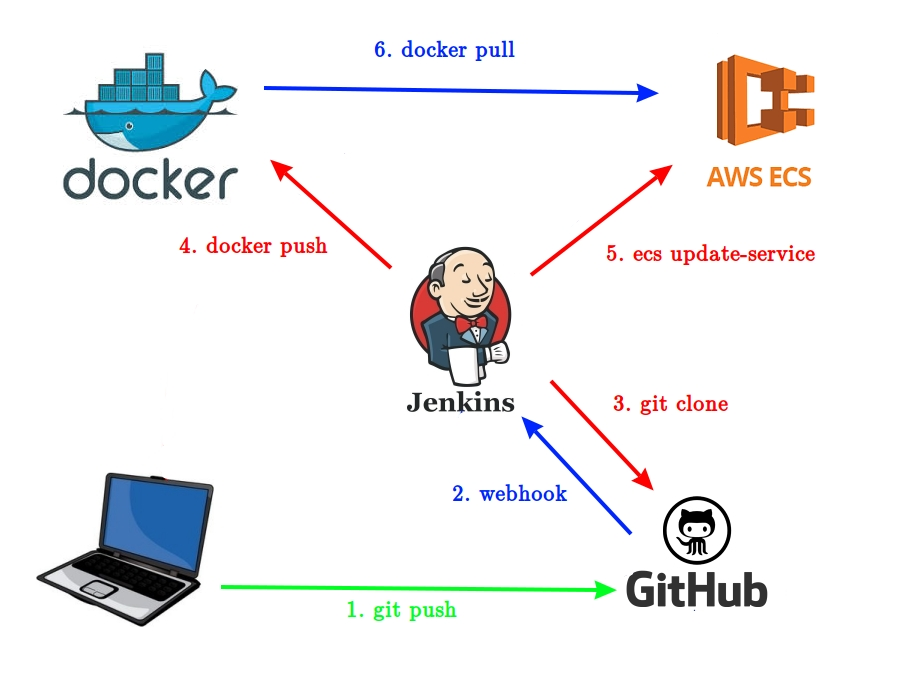
\includegraphics[scale=0.5,keepaspectratio]{cicd}
		\label{fig:cicd}
	\end{figure}

	\subsection{Documentation \& Testing}
  Documentation for the systems API is provided using Swagger. Swagger uses \textit{yaml} or \textit{json} files to document API endpoints, providing functions descriptions, parameters, possible responses and examples. Using the Swagger UI tool, the documented endpoints can then be visualized on the fronted of the web app \citep{swagger}.
  
  \begin{figure}[H]
    \setlength{\belowcaptionskip}{15pt plus 3pt minus 2pt}
    \caption{Some of the Systems API Endpoints}
    \centering
    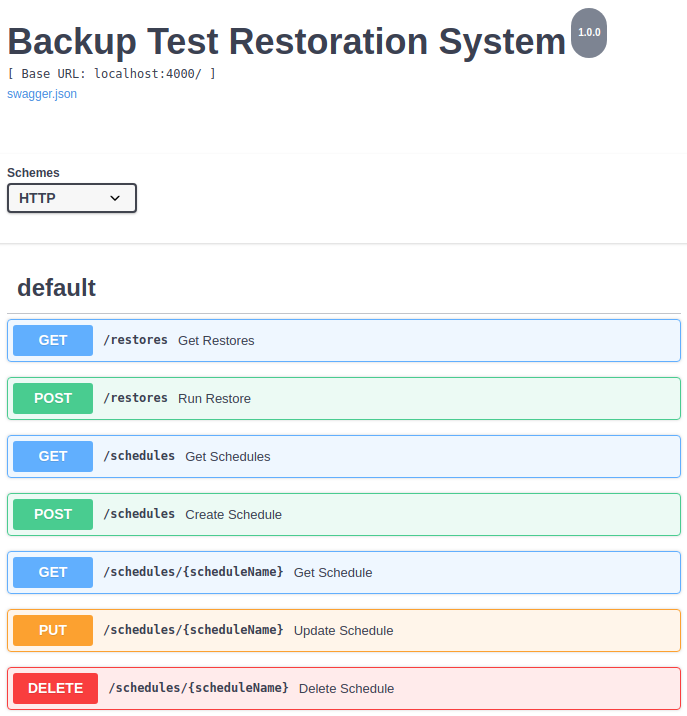
\includegraphics[scale=0.5,keepaspectratio]{api-endpoints}
    \label{fig:api-endpoints}
  \end{figure}
  
  
  By expanding any of the endpoints shown in \autoref{fig:api-endpoints}, the full documentation for that endpoints can be viewed. Along with providing the inbuilt documentation for the system, the Swagger UI tool also allows the user to test the endpoints, either using the sample data provided by the documentation or user input data. A sample of this can be seen in \autoref{fig:api-sample}. Thus, full testing the system's API can be completed using Swagger.
  
  \begin{figure}[H]
    \setlength{\belowcaptionskip}{15pt plus 3pt minus 2pt}
    \caption{The Documentation for the \textit{Run Restore} Endpoints}
    \centering
    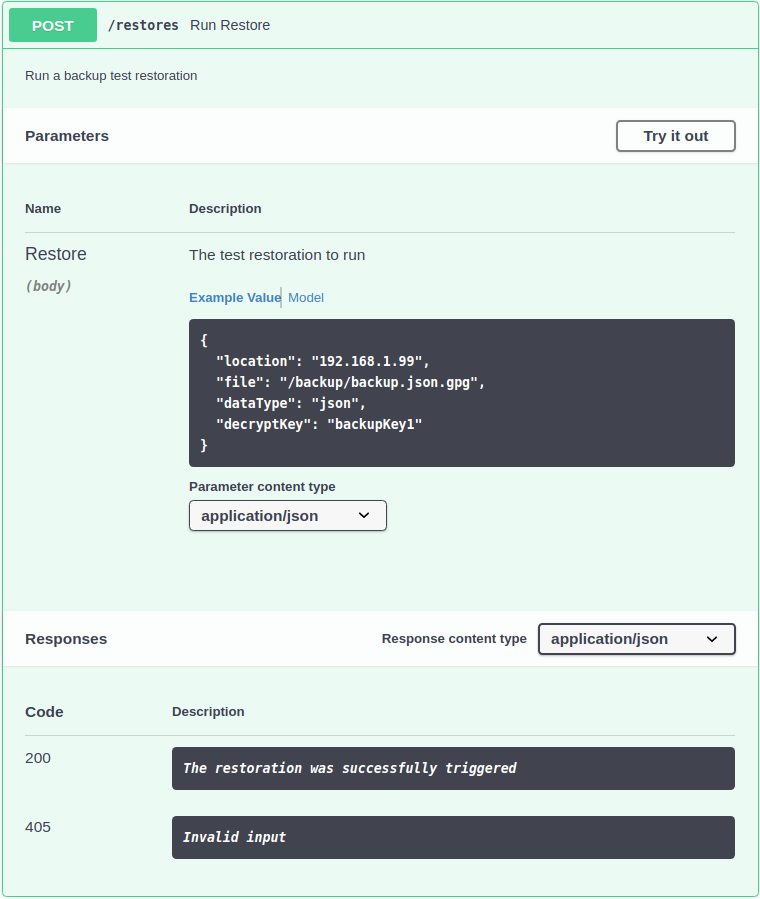
\includegraphics[scale=0.5,keepaspectratio]{api-sample}
    \label{fig:api-sample}
  \end{figure}
	
	\subsection{Completion and Handover}
	Due to the goal driven and iterative aspects of Agile methodology, a clear idea of a completed project is required. This will provide the final goal to work towards and a clear understanding of when this goal is reached. Accordingly, a \textit{Definition of Done} is a a key element of Scrum \citep{panchal}. The design methodology for this project will have the following stipulations:
	
	\noindent The \textit{Definition of Done} for each sprint will be as follows:
	
	\begin{itemize}
		\item Each issue (user story) has been tracked within Jira.
		\item Each issue is implemented;
		\item Each code for each issue has been documented.
		\item A sprint review meeting has been held;		
	\end{itemize}
	
	\noindent The \textit{Definition of Done} for the project  will be as follows:
	
	\begin{itemize}
		\item User stories have been categorised as \textit{Functional Goals} and \textit{Stretch Goals} in an initial backlog refinement;
		\item All \textit{functional} user stories have been implemented with considerations made for \textit{stretch goals};
		\item All code committed to GitHub repository;
		\item All code documented;
		\item Latest image of web app deployed to ECS through CI/CD;
		\item Latest image available on Docker Hub registry;
		\item A working deployment of the entire system is running and available for demonstration.
	\end{itemize}
	 
	 \noindent The following deliverables will be required for completion of the project. 
	 \begin{itemize}
	 	\item Presentation of the project;
	 	\item Project report;
	 	\item Descriptive poster of project;
	 	\item Demonstrative video of project feature.
	 \end{itemize}
\section{Implementation}
	\subsection{Sprint 0}
		\subsubsection{Sprint Planning}
		As the initial sprint of the project this sprint was concerned with setting up and configuring CI/CD tools for the project. The main tool of the CI/CD process considered were a Jenkins build server to continuously build and deploy the code and SonarQube to test code coverage and quality. Given the agile developments methodology was important to implement these steps early in the project and therefore they were undertaken during the initial sprint.

		\subsubsection{Sprint Review}
		The following goals were achieved:
		\begin{itemize}
			\item A Jenkins build server was deployed to AWS;
			\item An AWS ECS instance to run the web app was deployed;
			\item A skeleton React app was created with a defined Dockerfile to build image of the app;
			\item A Jenkins pipeline was created to build the image of the app and deploy it to AWS on every commit to GitHub;
			\item On account on SonarCloud was created, a cloud based service of SonarQube. 
		\end{itemize}
		
		\subsubsection{Sprint Retrospective}
		\textbf{What did we do well?}
		\begin{itemize}	
			\item CI/CD process has been set-up and implemented.
		\end{itemize}
		
		\noindent\textbf{What could have been done better?}
		\begin{itemize}
			\item Story Points have not been allocated to tickets;
			\item Breakdown of backlog could be improved, better utilising Epics, Issues and Subtasks.
		\end{itemize}
		
		\noindent\textbf{Actions}
		\begin{itemize}
			\item Rob Shelly to further refine the product backlog;
			\item Rob Shelly to add story points to tickets on backlog.
		\end{itemize}
		
		\subsubsection{Personal Reflection}
		This sprint highlighted the need for story points as the lack of such has meant there is not burndown chart for the sprint. Adding story points along with a well refined and organised backlog will allow for better sprint planning in the future.

	\subsection{Sprint 1}
		\subsubsection{Sprint Planning}
		The planning around for this session was based on the existing Jenkins Jobs created for \note[id=RB]{for what?} during the prototyping process. These jobs need to exist on the Jenkins server when the system is initially deployed/installed by a user. I.e, the user does not create these jobs.
		Therefore, these jobs need to be created during the installation process. This sprint focused on creating \textit{yaml} files for these jobs which can be used by \textit{Jenkins Job Builder} \added[id=RB, remark="show acronym in brackets the first time you use it"]{(JJB)}to create the jobs during set-up. This also provided the ability to quickly recreate the jobs should the Jenkins Server crash during development.

		\subsubsection{Sprint Review}
		The \textit{yaml} files were created and tested for the following Jenkins jobs:
		\begin{itemize}
			\item Deploy: Spins up a restoration server in AWS (i.e. a server with the correct DBMS installed)
			\item Decrypt:  Moves a backup file to a restoration server and decrypts it.
			\item Restore: Imports a backup file into the DBMS and performs a read of the data.
			\item Destroy: Destroys the restoration server after a successful backup restoration.
			\item Backup Restoration Pipeline:	Performs a full backup test restoration (using the above Jenkins jobs).
		\end{itemize}
		The sprint delivered on it's main focus of creating the \textit{yaml} files. However, \deleted[id=RB]{to} further tickets which would have built upon the prototype (displaying the result of the restoration) were not completed.

		\subsubsection{Sprint Retrospective}
		\textbf{What did we do well?}
		\begin{itemize}	
			\item Technically mastered the complexity of the project, have a
			vision and a direction to move towards;
			\item Backlog is very mature, the Minimum Viable Product (MVP) is almost visible;
			\item JJB was utilised and I now understand how Jenkins jobs
			work;
			\item Story Points were introduced and helped to guide the work.
		\end{itemize}
		
		\noindent\textbf{What could have been done better?}
		\begin{itemize}
			\item Burndown was inconsistent, consider taking smaller tickets;
			\item Domain knowledge in certain areas (JJB) was not as strong
			as I would have liked it to be, which slowed me down and
			was not reflective of the complexity I had awarded those
			tickets;
			\item Outward communication to the stakeholders (Leigh \& Paul)
			was not as good as it could have been.\note[id=RB]{Why do you say that? Maybe expand this point a little and say how you will improve communication with stakeholders.}
		\end{itemize}

		\noindent\textbf{Actions}
		\begin{itemize}
			\item Rob Shelly to get a draft of \deleted[id=RB]{your} wireframes to Leigh by next Monday;
			\item Rob Shelly to complete MVP plan for the backend system and include an API definition and CLI guide.
		\end{itemize}

		\subsubsection{Sprint Burndown}
		% TODO
		//TODO
		
		

		\subsubsection{Personal Reflection}\note[id=RB]{This section is good, well done.}
		I was happy with the progress of this sprint as I felt creating the \textit{yaml} files for the Jenkins jobs was an vital task, not only to enable an MVP to be packaged as a deployable system, but to provided an easy method of recreating the Jenkins jobs should there be a loss of AWS servers during development.
		
		This sprint also highlighted the importance of planning the sprint with respect to other college work to be completed in the given time frame. Although, this sprint was planned for two weeks, the entirety of the work was completed within a number of days during the later of two weeks. In future, if other college work will take precedence for a number of days, I may plan to delay beginning the sprint, allowing the final burndown chart to\deleted[id=RB]{t} better reflect the progress of work over the sprint.

	\subsection{Sprint n}

	\subsection{Sprint Metrics}
	% TODO
	TODO

	
\section{Summary}

  \subsection{Project Direction}
  
  The project at this points has succeeded in delivering an MVP to the product owners. However, development is not finished and is still ongoing. The current product backlog is shown in Figure (\textbf{TO DO} take product backlog picture after final sprint is complete).
  
  Current projections estimate that the project should complete it's backlog within two/three more sprints, at which point a fully implemented version of the product as set out by the project's aims and objectives. This projection can eb extrapolated from the cumulative dlow shart shown in \autoref{fig:flow} which shows the progression of tickets under the three categorires; \textit{To Do}, \textit{In Progress} and \textit{Done}.
  
  \begin{figure}[H]
    \setlength{\belowcaptionskip}{15pt plus 3pt minus 2pt}
    \caption{Cumulative Flow Chart}
    \centering
    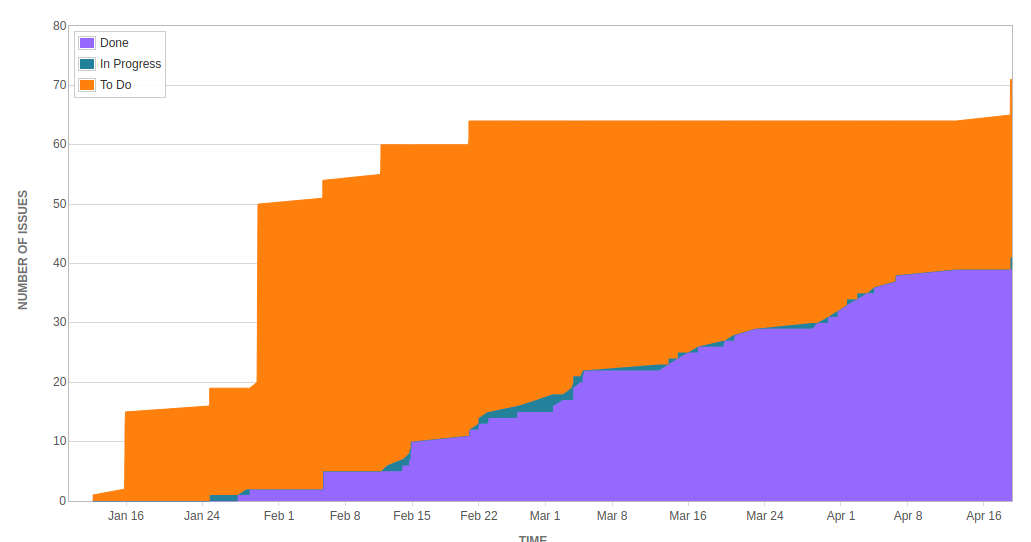
\includegraphics[width=\textwidth,keepaspectratio]{cumulative-flow}
    \label{fig:flow}
  \end{figure}
  
  This chart shows not only completion of work but also the discovery of new tasks and issues during the development  process, leading to and increase in the workload in the \textit{To Do} category. Of particular note in this chart is the significant increase in the workload that occurred in early February. This is reflective of the discussion and actions after an early retrospective with the product owners to focus separate the concerns of the backend API from the fronted UI. This resulted in intensive backlog refinement which included the creation of some new tickets.
  
  \subsubsection{Future Development}
  This project has been designed with future expansion of product features in mind. Indeed a noted aspect of this project is that it can currently test no relational data, but can be easily expanded to test relational data. This is facilitated by the modularity of the management servers tasks (created as Jenkins jobs) which can be interchanged as new tasks are added. For example:
  
  \begin{itemize}
    \item The task for restoring and reading data could be swapped with one which restores MySQL data instead of JSON.
    \item The decryption task (which use asymmetric cryptography) could be swapped with one which uses symmetric cryptography. 
  \end{itemize}
  Neither of these operations would affect other tasks and would be invisible to the end user.  The user could simply enter the correct setting at the dashboard and the necessary taskl would be \textit{chained} together using Jenkins Pipelines. 

	\subsection{Review}
  
  \subsubsection{Core Goals}
	This project delivered on it's core goals set out the the stakeholders. In relation to it's initial aims and objectives, the project has delivered the following aspects:
  
  \begin{itemize}
    \item \hyperref[ao1]{AO1:} An automated system for running a scheduling test restorations has been implemented:
    \item \hyperref[ao2]{AO2:} A notification system has been implemented to notify users of failed backups;
    \item \hyperref[ao3]{AO3:} The creation and destruction of the necessary infrastructure has been automated in order to reduce uptime and therefore also costs;
    \item \hyperref[ao4]{AO4:} Credentials have been stored and utilised in a secure manner and sensitive backup data has not been exposed;
  \end{itemize}
  
  The delivered product implemented three main components:
  \begin{itemize}
    \item A management server for the configuration and orchestration of the backup restores, implemented as a Jenkins server;
    \item A comprehensive ExpressJS API for interacting with the management server, abstracting the full configuration of Jenkins away from the user.
    \item A comprehensive frontend UI for users to use the API.
  \end{itemize}
  
  \subsubsection{Stretch Goals}
  The following stretch goals have been defined and remain on the product backlog for further development:
  
  \begin{itemize}
    \item \textbf{CLI:} Create a CLI for more advanced users who more comfortable or profficient in command lines to use the system withouht visiting the user dashboard.
    \item \textbf{User Authentication: } Implemtend a user system for the UI, allowing to be deployed to a webserver in a public domain and used to authenticate and authorised users.
  \end{itemize}
  

	\subsection{Learning Outcomes}
  This project has produced a number of learning outcomes.
  
  \subsubsection{Techinal Learning Outcomes}
  The following technical skills were gained or developed over the course of this project:
  
  \begin{itemize}
    \item Realised the benefits of the separation of frontend and backend through the development of a backend API and a frontend UI, emphasized through the product owners recommendation to complete one before the other as oppose to concurrently;
    \item Gained valuable insight into the containerisation of through researching the option of deploying multiple services to one or more containers;
    \item Learned about the CI/CD process through the implementation of a Jenkins CI/CD pipelines to build and deploy Docker images, a common software development practice in the industry when developing as part od a large team;
    \item Gained experience in developing a MEAN-stack application using ExpressJS, NodeJS and ReactJS having previously had little experience developing \textit{'full-stack'} applications;
    \item Reinforced the importance of API documentation and testing though the use of SwaggerUI;
  \end{itemize}
  
  \subsubsection{Non-Technical Learning Outcomes}
  There were also a number of  non-technical skills gained or developed over the course of this project.
  
  \begin{itemize}
    \item Learned about the benefits of project planning using Jira to define entire project workload early in the development stage.
    \item Experience was gained when dealing with a product owner. This including not only listening to their requirements and recommendation but also making decisions during development and updating the product owners accordingly.
    \item Learned how to correctly track workload and it's progress with Jira. The benefits of this were emphasised later in development when enough work had been completed to compile graphs which highlighted problem areas. This helped to keep the project focused on it's goal and meeting deadlines.
    \item Communication skills improved over the course of the project as a result of regular meetings with the scrum master and product owners.
  \end{itemize}
	
  \subsection{Personal Reflection}
  As the learning outcomes above show, I feel I have gained or improved a lot of skills while working on this project. Many of the skill I believed will be very beneficial to me in my future career. I found great satisfaction in completing and delivering the MVP as this is the largest and most comprehensive project I have undertaken.
  
  Personally I feel one of the most important learning outcomes of this project was the benefits of project planning. After the initial meeting with the product owners, at which points the main details of the project were outlined, there was a quite time consuming and tedious job of splitting the entire project in small tasks. These tasks were then added to Jira as tickets. The granularity at which this had to be done was something I had never completed before. In previous projects I would set out \textit{To Do} lists at a much higher level, with only a few items on the list. 
  
  However, the amount of time and effort put into creating these tickets and organising them into \textit{Epics} and \textit{Issues} proved to be hugely benefitial later on in the development phase. Having the tickets created that clearly defined all the steps required to implement each user story meant I never lost focus of what I was doing. Also on completing of any given task, there was no confusion or decisions needed as to what to do next. This was always easily determined due to clearly defined tickets and a well refined backlog.
  
  I also found the prototyping stage to be of huge benefit. Initially I was unsure as to whether the project would be technically feasible. In the past I would have determined this only though beginning development and hoping to overcome issues as they arise. However, the product owners' recommendation and help in identifying the key areas of uncertainty and defining \textit{proof of concepts} accordingly was a valuable lesson. This is a lesson I will certainly remember for future projects i.e. identify problem areas before development begins and investigate their feasibility with a \textit{proof on concept} prototype.
  
  Overall I found the project be greatly beneficial to my growth as a developer. Accordingly, I would deem the project to be a personal success with many valuable lessons and experiences.
  
  
  
  



\newpage
\renewcommand*{\bibfont}{\raggedright}
\bibliographystyle{plainnat}
\bibliography{bibliography/bibtex}

\end{document}


